%% ---------------------------------------------------------------------------
%%  UnionLabs — ACM MobiCom demo paper.
%%
%%  FORMAT per the MobiCom call for demos: 2 pages double-column US letter,
%%  fonts no smaller than 10pt, ACM template, plus ONE EXTRA PAGE FOR
%%  REFERENCES. Demo submissions are SINGLE-BLIND: authors are named.
%%
%%  Build:   make
%%  BEFORE SUBMITTING: fill the author block, then delete the \TODO line.
%% ---------------------------------------------------------------------------
\documentclass[sigconf,10pt]{acmart}

\usepackage{graphicx}
\graphicspath{{figs/}}
\usepackage{tikz}
\usetikzlibrary{positioning,arrows.meta,fit,backgrounds,calc}
\usepackage{xcolor}
\usepackage{balance}

\newcommand{\TODO}[1]{\textcolor{red}{\textbf{[TODO: #1]}}}
\newcommand{\code}[1]{\texttt{\small #1}}
%% Narrow columns + unbreakable \code{} spans overflow the measure; let TeX
%% stretch a little rather than run into the next column.
\emergencystretch=1.2em
\hyphenpenalty=100

%% --- venue block. MobiCom 2026: Austin, Texas, 26--30 October 2026. --------
\acmConference[MobiCom '26]{The 32nd Annual International Conference on Mobile
  Computing and Networking}{October 26--30, 2026}{Austin, TX, USA}
\acmYear{2026}
\copyrightyear{2026}
\setcopyright{acmlicensed}
%% \acmISBN{...} \acmDOI{...}  — add when ACM supplies them.

\setlength{\textfloatsep}{6pt plus 2pt minus 2pt}   % float <-> text (top/bottom-of-page floats)
\setlength{\intextsep}{5pt plus 2pt minus 2pt}      % float placed "here" [h]
\setlength{\floatsep}{6pt plus 2pt minus 2pt}       % between two stacked floats
\setlength{\abovecaptionskip}{3pt}                  % gap above a caption
\setlength{\belowcaptionskip}{1pt}                  % gap below a caption

%% acmart hard-codes the space around section headings (-.75\baselineskip
%% before, .25 after) inside \@startsection, so tightening it needs a patch:
\makeatletter
\renewcommand\section{\@startsection{section}{1}{\z@}%
  {-.55\baselineskip \@plus -2\p@ \@minus -.2\p@}%
  {.18\baselineskip}%
  {\ACM@NRadjust\@secfont}}
\makeatother

\renewcommand{\topfraction}{0.92}
\renewcommand{\floatpagefraction}{0.82}

\begin{document}

\title{UnionLabs: new agent, features, physical layers}

%% ---------------------------------------------------------------------------
%%  AUTHORS — fill in. Demos are SINGLE-BLIND, so real names belong here.
%%  acmart's \author/\email/\affiliation are fragile: plain text, no macros.
%% ---------------------------------------------------------------------------
\author{First Author}
\affiliation{%
  \institution{Institution}
  \city{City}
  \country{Country}}
\email{first@example.edu}

\author{Second Author}
\affiliation{%
  \institution{Institution}
  \city{City}
  \country{Country}}
\email{second@example.edu}

\author{Third Author}
\affiliation{%
  \institution{Institution}
  \city{City}
  \country{Country}}
\email{third@example.edu}

\begin{abstract}
Running a wireless learning experiment still means hand-assembling everything
around the algorithm: a radio stack, the wiring of every node, a testbed's
containers, and the ports between them. We present UnionLabs, a platform that
turns each of these into a designed, reusable part. An algorithm declares only
\emph{what to transmit} and \emph{what to receive}, and moves unchanged
between different physical layers. The wiring of a multi-node experiment is a
declarative file in which every link carries its own medium, per
direction---checked when it is read, not when it fails on the air. A shared
workspace carries one account's experiment state across testbeds that cannot
reach each other, and an agent turns any machine into a managed edge node,
exposing hardware to experiment containers only by the lab owner's permission.
In this demonstration, users create the experiment environment, visit the
remote desktop in the container, and test the algorithms over different
physical layers.
\end{abstract}

\begin{CCSXML}
<ccs2012>
<concept><concept_id>10003033.10003079.10003081</concept_id>
<concept_desc>Networks~Network experimentation</concept_desc>
<concept_significance>500</concept_significance></concept>
<concept><concept_id>10003033.10003079.10011672</concept_id>
<concept_desc>Networks~Network measurement</concept_desc>
<concept_significance>300</concept_significance></concept>
</ccs2012>
\end{CCSXML}
\ccsdesc[500]{Networks~Network experimentation}

\keywords{unionlabs, software-defined radio, wireless testbeds, experiment
orchestration, wireless applications.}

\maketitle

%% ===========================================================================
\section{Motivation}
%% ===========================================================================
An experiment that places learning inside the radio loop, federated averaging
over the air~\cite{mcmahan2017fedavg}, decentralized consensus over a
graph~\cite{lian2017dpsgd}, is easy to state and expensive to run. Shared
platforms have removed the hardware barrier~\cite{powder, colosseum}, and open
physical-layer stacks the waveform barrier~\cite{gnuradio, srslte}, but users
still need to understand the hardware code and link their algorithms to the
physical layer, writing hundreds of lines and spending days debugging. We
introduce UnionLabs, a platform that separates \emph{what an algorithm does}
from \emph{how the experiment is wired}.

%% ===========================================================================
\section{UnionLabs Design}
%% ===========================================================================
The new features of UnionLabs comprise four parts, each shown in its own
figure.

\begin{figure}[h]
\centering
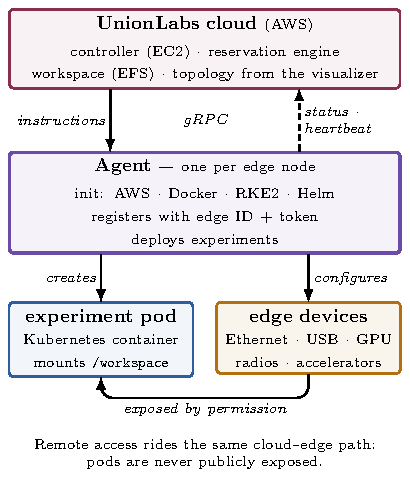
\includegraphics[width=0.65\linewidth]{fig-agent-col}
\caption{The UnionLabs Agent: middleware between the cloud services and the
physical testbed.}
\Description{The cloud on top, the agent in the middle connected by a gRPC
channel, and below it the experiment pod and the edge devices it exposes by
permission.}
\label{fig:agent}
\end{figure}

\textbf{The UnionLabs Agent.} The agent runs on every edge node---a server,
workstation, or laptop (Figure~\ref{fig:agent}). At install it prepares AWS,
Docker, an RKE2 Kubernetes server, and Helm, and registers the node with a
unique edge ID and token. It then holds a gRPC channel with the cloud, where
the controller, the reservation engine, and the topology uploaded through the
testbed visualizer live: instructions flow down, status and heartbeats flow
up. For each scheduled experiment, the agent creates a Kubernetes pod that
mounts the shared workspace, configures the node's devices---Ethernet, USB
radios, GPUs---and exposes them into the pod only by the lab owner's
permission. Remote access rides the same cloud--edge path, so pods are never
publicly exposed.

\begin{figure}[h]
\centering
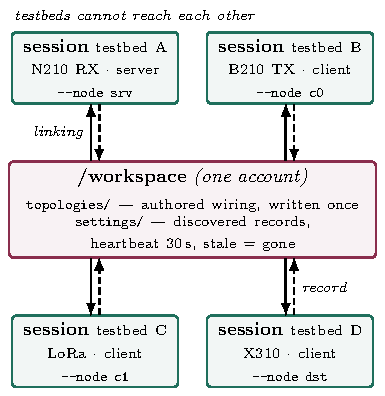
\includegraphics[width=0.65\linewidth]{fig-shared-workspace-col}
\caption{The shared workspace across sessions under a single account.}
\Description{A central workspace box linked to four session boxes on
different testbeds; wiring flows to each session and records flow back.}
\label{fig:workspace}
\end{figure}

\textbf{Deployment on Shared Testbeds.} Every session of one account mounts
the same \code{/workspace}, even when their testbeds cannot reach each other
(Figure~\ref{fig:workspace}). Its \code{topologies/} folder holds the
authored wiring, written once by the experimenter; its \code{settings/}
folder holds the record each session publishes about itself, refreshed on a
30-second heartbeat and dropped when stale. The wiring links every
session---here an N210 server, a B210 client, a LoRa client, and an X310
client on four testbeds---and their records flow back into the same folders.

\begin{figure}[h]
\centering
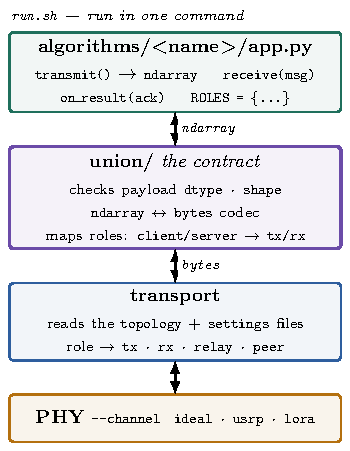
\includegraphics[width=0.6\linewidth]{fig-union-api-col}
\caption{The union API. A uniform path to link the users' algorithm with our
embedded wireless system.}
\Description{Four stacked blocks connected by double arrows: the experiment
file, the union contract, the transport, and the PHY.}
\label{fig:overview}
\end{figure}

\textbf{Algorithm Contract.} The user's algorithm writes two functions,
\code{transmit()} and \code{receive(msg)}, and nothing else
(Figure~\ref{fig:overview}). Beneath it, the union layer validates each
payload and converts it between \code{ndarray} and bytes; the transport
reads the topology and settings files and gives the node its
role---\code{tx}, \code{rx}, \code{relay}, or \code{peer}; and
\code{-{}-channel} selects the physical layer that carries the bytes. The
same path runs in both directions, so an algorithm moves between physical
layers by changing one flag, with no code change.

\textbf{Wiring as a File.} A topology is a declarative document naming each
node, its role in the algorithm's own vocabulary, the radio it owns, the
ports it listens on, and the links between nodes; each node is launched with
the same file and its own identity, and a typed flag still wins. One command
checks the whole of it, walking 44 command-line flags and 82 topology
settings from the text a user types to the object each configures.

\textbf{Per-Link, Per-Direction Media.} Each link states how it is carried,
and its two directions may differ: a rig with one transmit-capable and one
receive-only radio has exactly one RF path, so the reply must return over
TCP/IP, and a chain may change medium half way through. Wirings that cannot
run are refused when read---a transmitter with no transmit chain, two nodes
claiming one port, or a reply asked to travel over the air.

\begin{figure}[h]
\centering
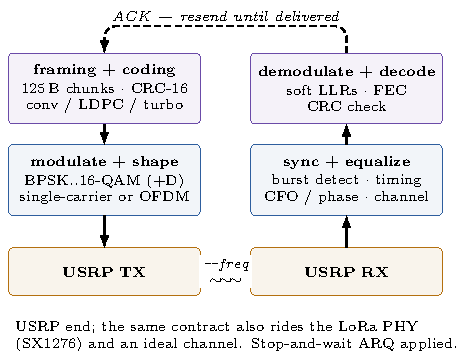
\includegraphics[width=0.8\linewidth]{fig-phy-pipeline-col}
\caption{The PHY design, stop-and-wait ARQ applied.}
\Description{Transmit chain of framing, coding and modulation on the left;
receive chain of synchronization, equalization and decoding on the right; an
ACK arrow closes the loop.}
\label{fig:phy}
\end{figure}

\textbf{PHY Codes.} The transmit side frames each payload, protects it with
a selectable channel code, and modulates it with a selectable scheme over a
single-carrier or OFDM waveform (Figure~\ref{fig:phy}). The receive side
synchronizes to the burst, corrects carrier and phase, equalizes the channel,
and decodes down to an integrity check. Stop-and-wait ARQ closes the loop: a
chunk is resent until its acknowledgement arrives, over TCP or a second RF
path. Modulation, coding, synchronization, waveform, gains, and the carrier
frequency are all selectable per experiment, and the same contract also rides
the LoRa PHY and an ideal, radio-free channel.

%% ===========================================================================
\section{Demonstration}
%% ===========================================================================
The demonstration shows each designed part working, live: visitors onboard a
machine, open the experiment container, and run one algorithm over different
physical layers. Each step takes two to three minutes.

\textbf{Onboarding an Edge Node (Agent).} A machine is enrolled on the spot:
the agent prepares its environment, registers it, and its heartbeat appears
on the platform. Once an experiment is scheduled, the visitor opens the
container's remote desktop through the cloud--edge path.

\textbf{One Workspace Across Testbeds.} From that desktop, the visitor edits
a wiring file in \code{/workspace} and sees the same file from a session on
a remote testbed, together with the records of the nodes that are live.

\textbf{One Algorithm, Different Physical Layers.} A learning algorithm runs
first with no radio, then over real radios by changing one flag. Visitors
watch delivery, retransmissions, and the airtime each round costs.

\textbf{Rewiring, and Refusal.} A multi-hop experiment changes its
medium---over the air or over the network---as the visitor edits one field. A
wiring that cannot run is refused when it is read, naming the node at fault.

%% Page-limit machinery removed while everything is being assembled: restore
%% \balance + \clearpage here when trimming to 2-pages-plus-references.
{\small
\bibliographystyle{ACM-Reference-Format}
\bibliography{bib}
}

\end{document}
